\chapter{Higher Genus Surfaces}
In this chapter, we construct exotic surfaces with arbitrary genus. We discuss how to adapt the proofs we have seen in the previous chapters to the positive genus case. \\ \\

Below, we present the final form of the main theorems of chapters 3 and 4.
\begin{thm}Let $g \geq 0$. There exist infinitely many transverse knots in $(\s^3, \xi_{st})$, each bounding a pair of exotic, genus $g$, symplectic surfaces in $(\B^4, \omega_{st})$.
\end{thm}
\begin{thm} \label{ulti} Let $g \geq 0$. There exist infinitely many convex symplectic $4$-manifolds containing a pair of exotic, closed, symplectic, genus $g$ surfaces.
\end{thm}




We begin by proving the non-closed case. Instead of constructing such surfaces from scratch, we will attach bands to the previously found exotic disks (i.e., perform the connected sum with a genus-$g$ surface).
\section{Holomorphic Curves Bounded by $\torus$}
In this section, we construct a genus-$g$ holomorphic \footnote{The usefulness of the holomorphic structure will become evident in the subsequent steps.} curve embedded in $\B^4$, with $g>0$. 
Consider the holomorphic function $$
f: \C^2 \rightarrow \C
$$ $$
(z_1, z_2) \rightarrow z_1^2 + z_2^{2g+1}
$$
\begin{as} Let $S_{\epsilon}\subseteq\C^2$ be the radius $\epsilon$ sphere centered in $0$, and $V = f^{-1}(0)$. Then $$
V \cap S_{\epsilon} = \torus
$$
\end{as}
\proof
Let $(z_1, z_2) \in V \cap S_{\epsilon}$. Then the following equations hold: $$
|z_1|^2+|z_2|^2 = \epsilon
$$ $$
|z_1|^2 = |z_2|^{2g+1}
$$
Thus $|z_1|$ and $|z_2|$ are equal to two costants $c_1, c_2$. An easy computation shows that all the points of the form$$
(c_1e^{(2g+1)i\theta}, c_2e^{2\pi i+\frac{\pi i}{2g+1}}) \qquad \theta \in [0, 2\pi]
$$ satisfy both the equations defining $V$ and $S_{\epsilon}$. Hence the thesis.
\endproof
Now, since $\nabla f(z) \neq 0 \quad \forall z \neq 0$, we can deform $V$ into a smooth complex curve, defined as: $$
F_0 = \{z_1^2 + z_2^{2g+1} = \epsilon\}
$$
for some small $\epsilon > 0$.
\begin{obs}  $\partial F_0 = \torus$ and $F_0$ has genus $g$, as required.
\end{obs}
Let $h: F_0 \rightarrow \B^4$ be an embedding. \\
Complex curves in Stein $4$-manifolds carry a natural positive symplectic form given by
the pullback of $\omega_{\phi}$ via $h$ \cite{eliashberg2012stein}. 
\begin{note} Symplecticity of $F_0$ can also be proven via Lemma \ref{cob} and the following transverse link movie:
\begin{figure}[H]
    \centering
    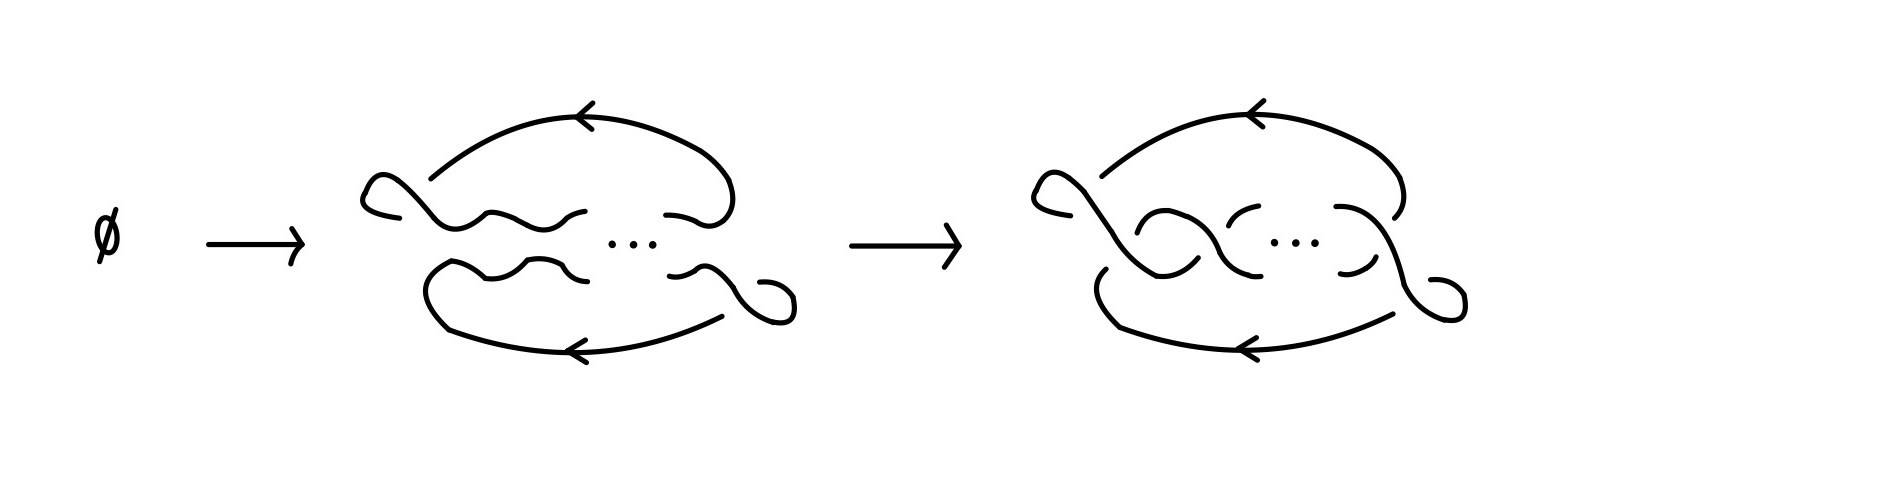
\includegraphics[scale=0.25]{figures/movie.jpeg}
    \caption{A transverse link movie for $F_0$}
    \label{fig:movie}
\end{figure}
\end{note}
Let $F = F_0 \natural D$ and $F' = F_0 \natural D'$ (where $D, D'$ are the exotic disks of Theorem \ref{prince}).
\begin{note} $\partial F = \partial F' = K_m \#\torus$ are transverse knots in $(\s^3, \xi_{st})$.
\end{note}
We claim that $F, F'$ is an exotic pair of genus $g$ symplectic surfaces.
Since $D$ and $D'$ are topologically isotopic, the same holds for $F$ and $F'$. \\ \\
To prove that $F, F'$ are symplectic, we observe that the connected sum of two knots can be achieved using the saddle move shown in Figure \ref{fig:moves}(b), and then use Lemma \ref{cob}.  \\ \\
It remains to show that $F$ and $F'$ are not smoothly isotopic (relatively to the boundary). We mimic the strategy used for the case $g=0$. 
Assume by contradiction that there exists a diffeomorphism $\varphi: \B^4 \rightarrow \B^4$ such that $\varphi(F') = F$. Hence $\varphi (K_m \# \torus) = K_m \# \torus$. 
We aim to prove that $J \subseteq \s^3 \setminus (K_m \# \torus)$ is fixed by $\varphi$, up to isotopy. To this end, we study the set of diffeomorphisms of $Y = \s^3 \setminus (K_m \# \torus)$, up to isotopy. 
\begin{lem} \label{techhh} Suppose that $m = 0$ or $m<<0$.
Then every self diffeomorphism of $\s^3 \setminus (K_m \# \torus)$ restricts to the identity on $\s^3 \setminus \inter$, up to isotopy.
\end{lem}
Unfortunately, $Y$ is not hyperbolic (so we can't use the same argument of Lemma \ref{technic}) . However, we can decompose $Y$ into simpler pieces.
In this section, we prove Lemma \ref{techhh} using the $JSJ$ decomposition tool, reducing the argument to that of Lemma \ref{technic}.
\\ \\
First, we briefly review the $JSJ$ decomposition following Hatcher's notes \cite{hatcher2002notes}. Let $Y$ be a $3$ manifold. 
\begin{defn}$Y$ is said to be irreducible if every embedded sphere $S \rightarrow Y$ bounds a ball $\B^3 \subseteq Y$. 
\end{defn}
\begin{ex} For every knot $K$, $\s^3 \setminus K$ is an irreducible manifold. In fact, every sphere bounds two balls in $\s^3$, one of which contains $\nu(K_m)$. Hence the other is contained in $\s^3 \setminus K$.
\end{ex}
\begin{defn}Let $F \rightarrow Y$ be an embedded surface other than $\s^2$ or $\D^2$.
$F$ is said to be incompressible if for each disk $D \subseteq Y$ with $D \cap F = \partial D$, there exists a disk $D' \subseteq F$ such that $\partial D = \partial D'$ (as in Figure \ref{fig:seifert}(a)).
\end{defn}
\begin{ex}\label{heart} Let $V$ be a unknotted torus, and let $P\subseteq V$ be an essential\footnote{It means that $P$ intersects every meridional disk} knot. Consider a diffeomorphism $h : V \rightarrow \nu(C)$. 
$$
S  (C, P) = h(P) \subseteq \nu(C)
$$
is called a satellite knot with companion $C$ and pattern $P$. \\
The torus $h(\partial V)$ is incompressible in the exterior of $S(C, P)$. \cite{schultens2014introduction}, cfr \cite{gabai1987foliations}. 
\end{ex}
The concepts of knot complements and $JSJ$ decomposition are intimately related; we refer the interested reader to \cite{budney2006jsj}. 
\begin{figure}[H]
    \centering
    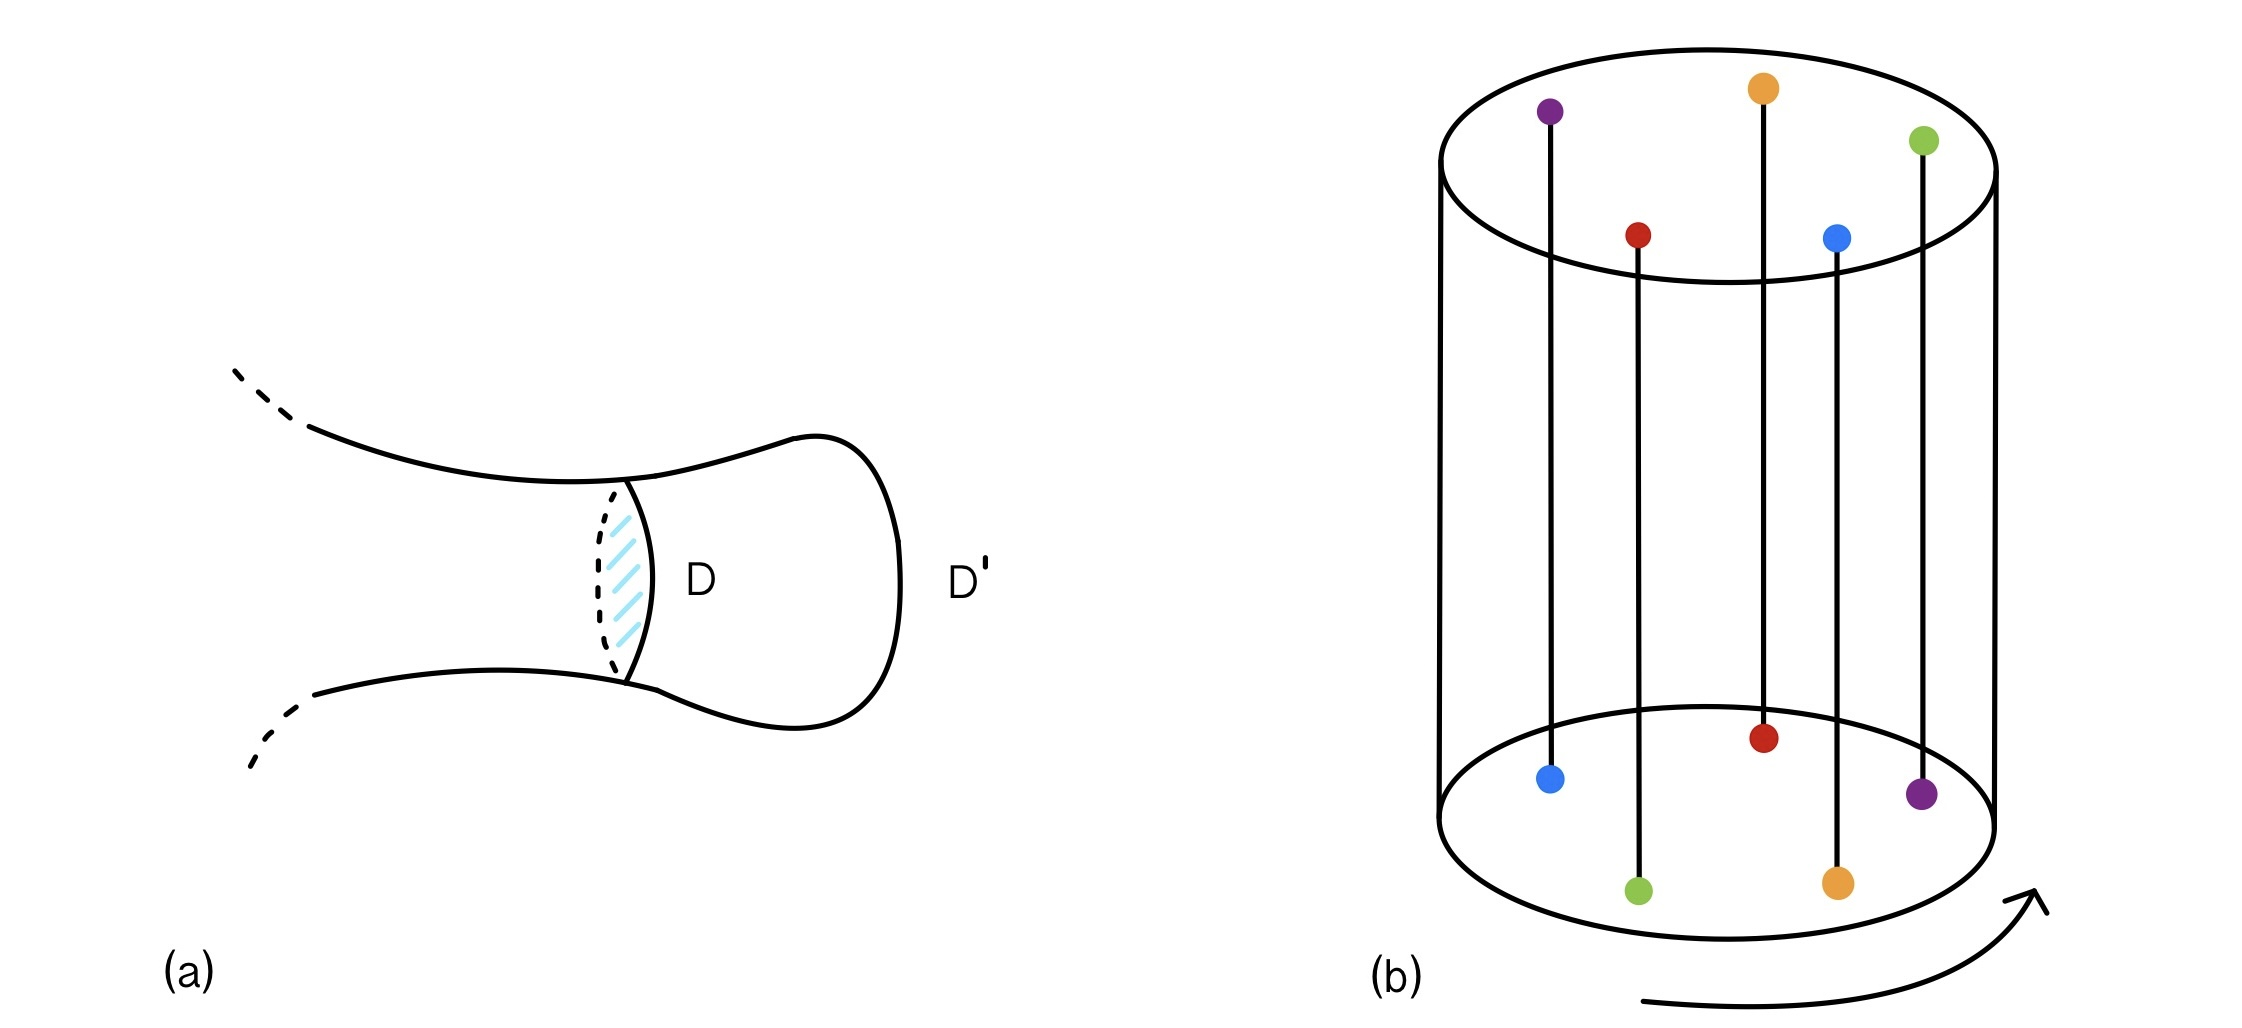
\includegraphics[scale=0.2]{figures/seifert.jpeg}
    \caption{An incompressible surface (a) and a Seifert fibered model of $\s^1 \times \D^2$ (b)}
    \label{fig:seifert}
\end{figure}
Now we describe the two building blocks for the decomposition. 
\begin{defn}Let $Y$ be an irreducible $3$ manifold. \\
(i) $Y$ is called atoroidal, if every incompressible torus $T^2 \rightarrow Y$
is isotopic to a component of $\partial Y$. \\
(ii) Let $p, q$ be coprime integers. A type $(p, q)$ model Seifert fibering of $\s^1 \times \D^2$ is a decomposition of $\s^1 \times \D^2$ into disjoint copies of $\s^1$ made as follow. We start with a cylinder $[0, 1] \times \D^2$ with fibers $[0, 1] \times \{x\} \quad x \in \D^2$. Then we glue the bottom $0 \times \D^2$ with the top $1 \times \D^2$ via a $\frac{2\pi p}{q}$ rotation (as in Figure \ref{fig:seifert}(b)). $Y$ is called Seifert fibered if it decomposes into disjoint copies of $\s^1$, and it is locally diffeomorphic to a model Seifert fibering of $\s^1 \times \D^2$. 
\end{defn}
\begin{ex}\label{sei1} The complement of a Hopf link $L$ in $\s^3$ admits a Seifert fibering. In fact, $\s^3 \setminus L \cong T^2 \times [0, 1]$.
\end{ex}
An important class of Seifert fibered $3$-manifolds are the complements of torus knots. 
\begin{prop}\label{sei2} Let $p\neq q$ be prime numbers. Then $\s^3 \setminus T_{p, q}$ admits a Seifert fibering.
\end{prop}
For a proof, consult \cite{martelli2016geometric} Proposition $11.2.5$. \\
Finally, we state the $JSJ$ decomposition theorem.
\begin{thm} \cite{jaco1978new}\cite{johannson1979homotopy}
Let $Y$ be a compact, irreducible, orientable $3$ manifold with toroidal boundary. Then $Y$ admits a minimal collection of disjoint, non-boundary parallel, incompressible tori $T = \{T_1, \dots T_k\}$, such that each component of $$
Y|T = Y \setminus (\nu(T_1)^{\mathrm{o}} \cup \dots \cup \nu(T_k)^{\mathrm{o}})
$$
is either atoroidal or Seifert fibered. Such collection is unique, up to isotopy. 
Moreover, for every diffeomorphism $\psi$ of $Y$, there exists a permutation $\sigma \in \mathfrak{S}_k$ such that $$
\psi(T_j) = T_{\sigma(j)}
$$
\end{thm}
With these tools in hand, we now prove Lemma \ref{techhh}. 
\proof Let $\varphi \in Diff(\s^3 \setminus K_m \# \torus)$.
We may view $K_m \# \torus$ as a satellite knot sitting inside $\nu(K_m)$. The torus $T = \partial \nu(K_m)$ is called a swallow-follow torus \ref{fig:swallow}(b), as it swallows $\torus$ and follows $K_m$ (which is depicted as a figure-eight knot for simplicity). Such torus is realized as the boundary of a component of $\s^3 \setminus (\nu(K_m) \cup S)$ (Figure \ref{fig:swallow}(a)), where $S$ is a decomposing sphere for $K_m \# \torus$. As discussed in Example \ref{heart}, $T$ is an incompressible torus in  $Y = \s^3 \setminus (K_m \# \torus)$. Thus we can decompose $Y$ along $T$ as: $$
(\s^3 \setminus \nu(K_m)) \cup_{\partial(\s^3 \setminus \mu) = T} (\s^3 \setminus \nu (\torus \cup \mu))
$$ 
where $\mu$ denotes a meridian\footnote{$\mu$ wraps around like $K_m$} of $\torus$. 
Similarly, $\s^3 \setminus (\torus \cup \mu)$ decomposes into two $JSJ$ pieces: $\s^3 \setminus \torus$ and the complement of a Hopf link. By Example \ref{sei1} and Proposition \ref{sei2}, the latter pieces are Seifert fibered, therefore they can't support a hyperbolic structure. Up to isotopy, we can assume that $\varphi(T) = T$, thus by uniqueness of the $JSJ$ decomposition, we conclude that $$
\varphi(\s^3 \setminus K_m) = \s^3 \setminus K_m
$$
Hence the thesis follows from Lemma \ref{technic}.
\endproof
\begin{figure}[H]
    \centering
    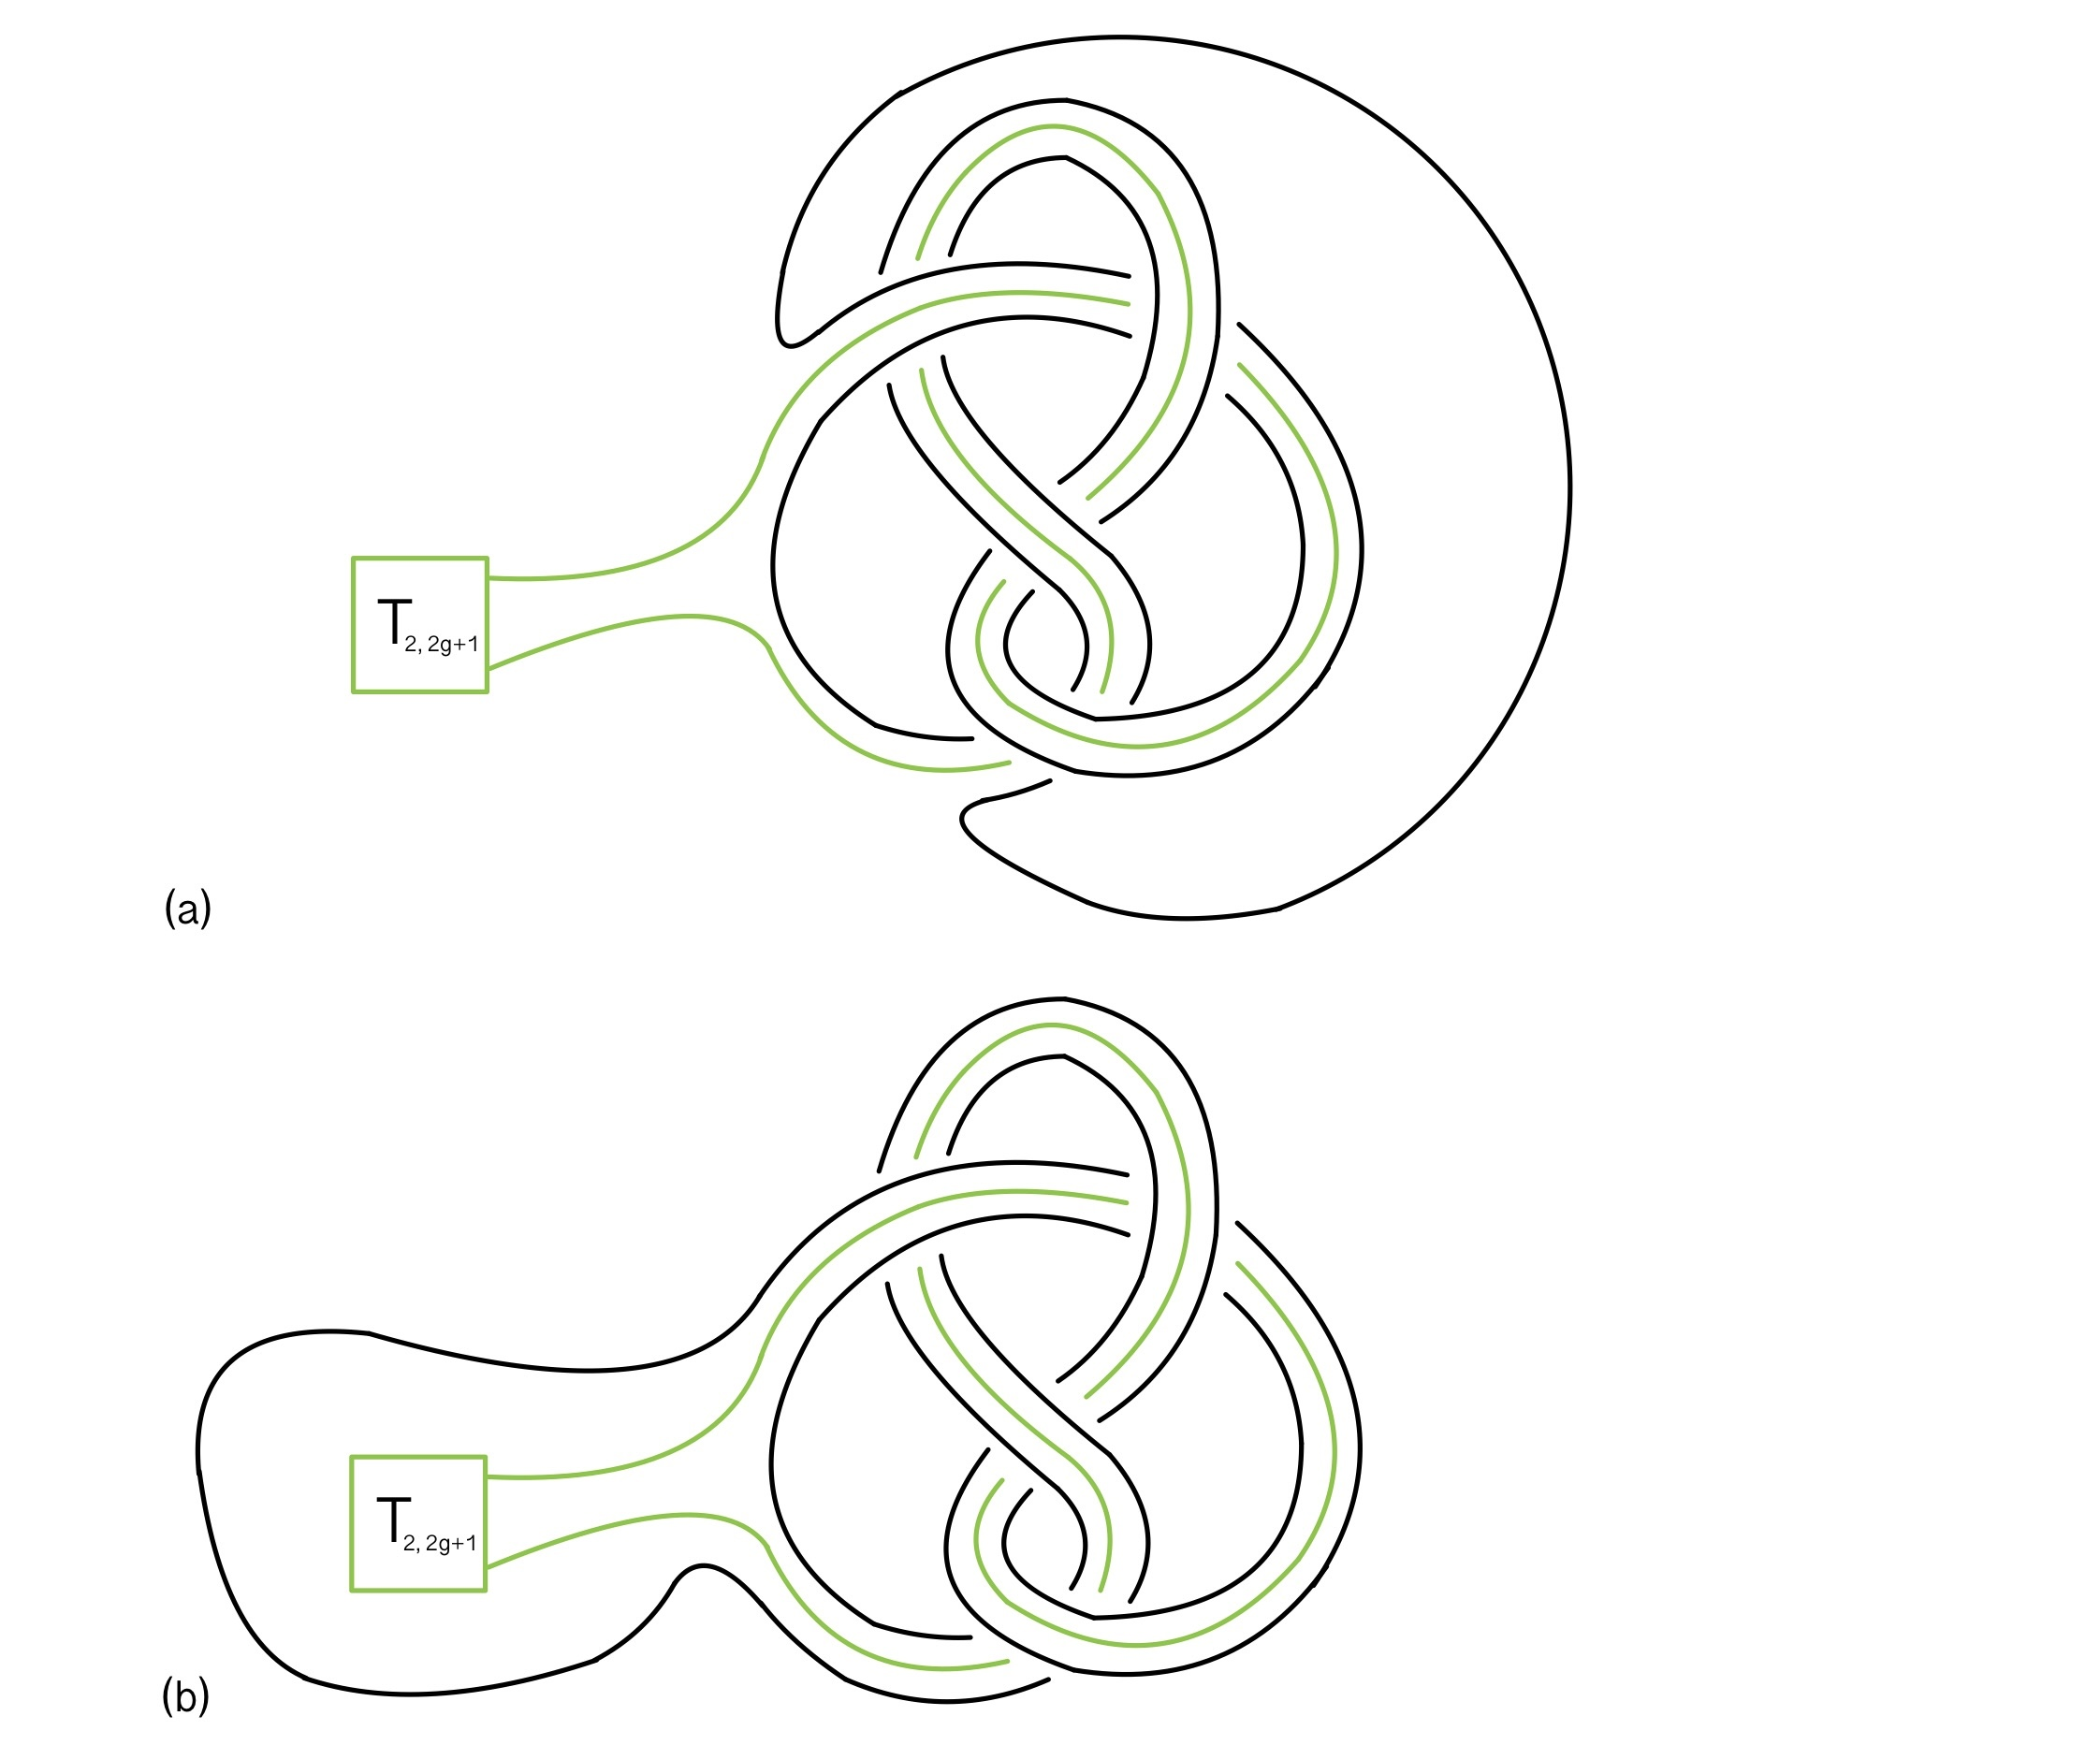
\includegraphics[scale=0.25]{figures/swallow.jpeg}
    \caption{A swallow-follow torus}
    \label{fig:swallow}
\end{figure}
As in the proof of \ref{prince}, $J$ bounds a disk $\mathfrak{D}'$ disjoint from $D'$.
By Lemma \ref{techhh} $$
\varphi(\mathfrak{D}') = \mathfrak{D} 
$$
is a disk bounded by $J$, which is contained in $\estd$.
Next, we aim to obstruct the existence of $\mathfrak{D}$, by analyzing a lift $\mathfrak{\tilde{D}}$ in the double branched cover $\Sigma(\B^4, F)$.
The existence and uniqueness of $\Sigma(\B^4, F)$ is proved in \cite{akbulutKirbyBranchedCovers}. The following Proposition ensures that $\Sigma(\B^4, F)$ is a Stein $4$-manifold.
\begin{prop}The following hold: \\
(i) $\Sigma(\B^4, D\natural F_0) = \Sigma(\B^4, D) \natural \Sigma(\B^4, F_0)$ \\
(ii) $\Sigma(\B^4, F_0)$ admits a Stein structure, \\
(iii) $\Sigma(\B^4, F)$ admits a Stein structure.
\end{prop}
\proof 
The first claim is straightforward from the definition of branched cover and the procedure to build it. \\
To prove (ii), we use the fact that a branched cover of $\B^4$ along an embedded holomorphic curve is analytic \cite{grauert_remmert_stein}. Then Theorem $3$ of \cite{loi_piergallini_stein} implies that $\Sigma(\B^4, F_0)$ is a Stein surface. \\
The last assertion follows from Gompf's standard form. In fact performing the connect sum corresponds to adding a $1$-handle.
\endproof
As the diagram of $\Sigma(\B^4, D)$ in Gompf's standard form is a portion of that of $\Sigma(\B^4, F)$, the final argument can be repeated verbatim. \\ \\
\section{Closed Case}
In this final section, we prove Theorem \ref{ulti}. As the proof is completely analogous to the proof of Theorem \ref{king}, we will only discuss the key changes. \\ \\
\proof
We consider $X_n = X_n(K \# \torus)$ as the ambient $4$-manifold. Let $G, G'$ be closed surfaces obtained by capping off $F, F'$ with the core of the $2$-handle in $X_n$. By Theorem \ref{hymn}, if $$
n \leq TB(K_m \# \torus)\footnote{This value is finite and does not depend from $m$ because $K_m$ has a Legendrian realization with $tb = -2$} - 1
$$

$X_n$ admits a convex symplectic structure. \\ Moreover, by Proposition \ref{tool4}, we can assume, up to isotopy, that $G, G'$ are symplectic in $X_n$. \\
It is straightforward to see that $G$ and $G'$ are topologically isotopic. \\
It remains to prove that they are not smoothly isotopic. Suppose, by contradiction, there exists $\varphi$, a self diffeomorphism of $\B^4$, such that $\varphi(G') = G$. \\
Next, we aim to show that $J \subseteq \partial X_n$ is fixed by $\varphi$, up to isotopy.
To this end, we prove an adapted version of Lemma \ref{tool8}, using again the $JSJ$ decomposition. 
\begin{lem} Let $n<<0$ and either $m<<0$ or $m=0$. Then every self diffeomorphism of $\partial X_n= \s^3_n(K_m \# \torus)$ restricts to the identity on $\s^3 \setminus \inter$, up to isotopy.
\end{lem}
\proof
First, we notice that $\partial \nu(K_m)$ defines an incompressible torus embedded in $\partial X_n$. Therefore $\s^3_n(K_m \# \torus)$ splits along $T$ into two $JSJ$ pieces, one of which is clearly $\s^3 \setminus K_m$. 
\begin{cla} The other piece is diffeomorphic to $\s^3 \setminus \torus$.
\end{cla}
In fact, the latter piece can be obtained by removing a meridian $\mu$ (of $\torus$) from $\s^3_n(\torus)$. Such meridian is glued to $n\mu+\lambda$ which is isotopic to $\torus$, the core of the surgered torus. \\
Thus $\partial X_n$ is decomposed as $$
\partial X_n|_T = (\s^3 \setminus K_m) \cup (\s^3 \setminus \torus)
$$
Recall that $\s^3 \setminus K_m$ is the only hyperbolic piece, as the other is Seifert fibered. Up to isotopy, every diffeomorphism of $\partial X$ preserves $T$ and restricts to a self-diffeomorphism of $\s^3 \setminus K_m$. Hence the thesis follows from Lemma \ref{technic}.
\endproof
Therefore $\varphi (\mathfrak{D'}) = \mathfrak{D}$ is a disk bounded by $J$ and disjoint from $G$. Next, we build the double branched cover of $X_n$ along $G$, using the same techniques employed in the proofs of Lemma \ref{warietto} and Theorem \ref{wario}. In particular, $$
\Sigma(X_n, G) = \Sigma(\B^4, F) \cup H_2
$$
with the $2$-handle attached along $\tilde{L}$, the lift of $K_m\# \torus$, with framing $\frac{n}{2}$. By Eliashberg's characterization theorem, if $$
n \leq TB(\tilde{L})-1
$$
$\Sigma(X_n, G)$ admits a Stein structure\footnote{As $n$ varies, using a sequence of negative stabilizations, we can always obtain a Legendrian realization of $\tilde{L}$ with $tb-1 = n$.}. From this point onward, the proof can be reproduced verbatim.
\endproof